% status: 0
% chapter: TBD

\title{Location based crime data search and analysis with Spark UDF}


\author{Kadupitiya Kadupitige}
\orcid{1234-5678-9012}
\affiliation{%
	\institution{Indiana University}
	\streetaddress{Smith Research Center}
	\city{Bloomington} 
	\state{IN} 
	\postcode{47408}
}
\email{jasakadu@iu.edu}

\author{Gregor von Laszewski}
\affiliation{%
  \institution{Indiana University}
  \streetaddress{Smith Research Center}
  \city{Bloomington} 
  \state{IN} 
  \postcode{47408}
  \country{USA}}
\email{laszewski@gmail.com}


% The default list of authors is too long for headers}
\renewcommand{\shortauthors}{G. v. Laszewski}


\begin{abstract}
This paper provides a sample of a \LaTeX\ document which conforms,
somewhat loosely, to the formatting guidelines for
ACM SIG Proceedings.
\end{abstract}

\keywords{hid-sp18-409, Crime data analysis, MapReduce, Google Maps, 
spark UDFs}


\maketitle


\section{Introduction}

A crime is generally defined as an act punishable by law and is one of
the dangerous factors for any
country\cite{hid-sp18-409-agarwal2013crime}. It is impossible to find
a country with a crime- free society due to complex causes such as
poverty, parental neglect, low self-esteem, alcohol, drug abuse and
etc~\cite{hid-sp18-409-bharathi2014survey,
hid-sp18-409-kiani2015analysis}.  Inspired by the big data revolution,
the historical way of crime solving and prevention has greatly
influenced and improved by the help of state-of-the-art data analytic
tools and machine learning research. Law enforcement officers have
started involving more data analytic expertises to speedup the crime
solving process highlighting that, it is an interdisciplinary research
area.

According to Chicago Police Department, crime prevention is important
and much more difficult to handle than crime solving for law
enforcement agencies~\cite{hid-sp18-409-www-cpd}. Law enforcement
officers could identify crime prone areas or suspicious activities
even before a crime is committed with the aid of pattern recognition
and big data analysis~\cite{hid-sp18-409-nath2006crime,
hid-sp18-409-gera2014city}.  According to the Los Angeles Police
Department (LAPD) and Chicago Police Department (CPD), whenever a
crime was committed somewhere, more crimes are likely to be occurred
in a nearby area, and the patterns of those criminal activities could
be identified through big data analysis~\cite{hid-sp18-409-www-cpd,
hid-sp18-409-www-lapd}. However, crime prevention could be so much
effective if there is an easy way to check the crime prone areas so
that people could be aware the of crime prone areas.

As inspired by the requirement to raise the awareness of crime prone
areas, we implement a location based crime search website where people
can find crimes happened near a particular geographical location (in a
vicinity area) for a given GPS coordinates. For this project, we have
selected a dataset which includes the crime information from 2001 to
current date in Chicago city~\cite{hid-sp18-409-www-data.gov}. We
further analyze this crime dataset using the crime type and timestamps to
identify the trends of crime types for a particular
geographical area. One applicational use of this project would be a
user trying to buy a new house and he may like to do a background
search on criminal activities around the geographical area for safety
concerns.

The organization of this project report is as follows. In section II,
a literature review on existing crime data analyses and crime
reporting web services are presented. Section III provides a
methodology followed in this project while section IV elaborates the
results and discussion. A summary about the project paper is provided
in section V.

\section{Literature Review}
The recent research and development in crime data investigation area
could be broadly categorized into two categories; analysis of
criminology~\cite{hid-sp18-409-agarwal2013crime,
hid-sp18-409-bharathi2014survey, hid-sp18-409-kiani2015analysis,
hid-sp18-409-nath2006crime, hid-sp18-409-gera2014city} and
applicational development of crime data visualization
platforms~\cite{hid-sp18-409-www-spotcrime,
hid-sp18-409-www-crimereports, hid-sp18-409-www-mylocalcrime,
hid-sp18-409-www-crimemapping}. Analysis of criminology data could be
further categorized into crime control and crime
suppression~\cite{hid-sp18-409-agarwal2013crime}. There exists many
research focused on analyzing crime data based on different
methodologies such as kmeans cluster
analysis~\cite{hid-sp18-409-gera2014city, hid-sp18-409-nath2006crime,
hid-sp18-409-agarwal2013crime}, time series
analysis~\cite{hid-sp18-409-wei2006time}, variational data mining
techniques~\cite{hid-sp18-409-chen2004crime}, geographical analysis
using using statistical techniques~\cite{hid-sp18-409-santos2016crime}
and etc. This study experiments combinations of these techniques to
build a crime data investigation platform and hence, they are
discussed in this section.

Agarwal et al.~\cite{hid-sp18-409-agarwal2013crime} have investigated
a comprehensive crime data analysis to identify the crime patterns and
predict crimes based on spatial data distribution of existing data
using kmeans clustering based approach and rapid miner tool. They have
only focused on homicide crime type and plotted the number of reported
crimes with respect to year for different clusters. This analysis had
helped them to conclude that homicide is decreasing from 1990 to 2011
in in England and Wales~\cite{hid-sp18-409-agarwal2013crime}.
Following Agarwal~\cite{hid-sp18-409-agarwal2013crime}, Kiani et
al.~\cite{hid-sp18-409-kiani2015analysis} have also studied the same
dataset to improve the clustering approach by assigning weights to the
features in the dataset and using Genetic Algorithm (GA) to optimize
the Outlier Detection using the same rapid miner tool. Gera et
al.~\cite{hid-sp18-409-gera2014city} have studied the possibility of
profiling the crimes using cluster analysis. Gera et
al.~\cite{hid-sp18-409-gera2014city} have analyzed all type of crimes
happened in Delhi police commission as well as through National Crime
Records Bureau (NCRB), Delhi, India. They have created a crime
database by interviewing concerned officers, through semi-structured
interviews, group discussion, participant observation, documentation
analysis and questionnaires in Delhi region to perform two types of
crime profiling based on types of crimes and types of areas. Finally
an association between two profiling methods were identified using
weka data mining tool. Similarly, Nath et
al.~\cite{hid-sp18-409-nath2006crime} also applied several clustering
algorithms to identify the association in crime data taken from
sheriff’s office in the city of New Orleans. They have also used a
semi-supervised learning technique for knowledge discovery from the
crime records and to help increase the predictive accuracy in the
crime data classification task.

Extensive time series analysis on Philadelphia crime data has been studied by Wei et al.~\cite{hid-sp18-409-wei2006time}. They have compared stationary and non stationary models, nonseasonal and seasonal models, intervention and outlier models, transfer function models, regression time series models, vector time series models, and their applications using the crime data. They have further elaborated the procedures of time series analysis including parameter estimation, diagnostic checks, forecasting, and inference using autoregressive conditional heteroscedasticity model and generalized autoregressive conditional heteroscedasticity model~\cite{hid-sp18-409-wei2006time}. 


\section{Methodology}
As described in the literature review, most of the research on crime data investigation focused on analyzing crimes by type of the crimes, time series information and geographical location. These techniques could be extended to a great extent for our crime data framework. In this section, we describe the data acquisition, data preprocessing, technology usage and implementation details of individual modules based on python implementation. Figure \ref{fig:overview} shows the suggested framework for crime data analysis and visualization.

\begin{figure}[htb]
	\centering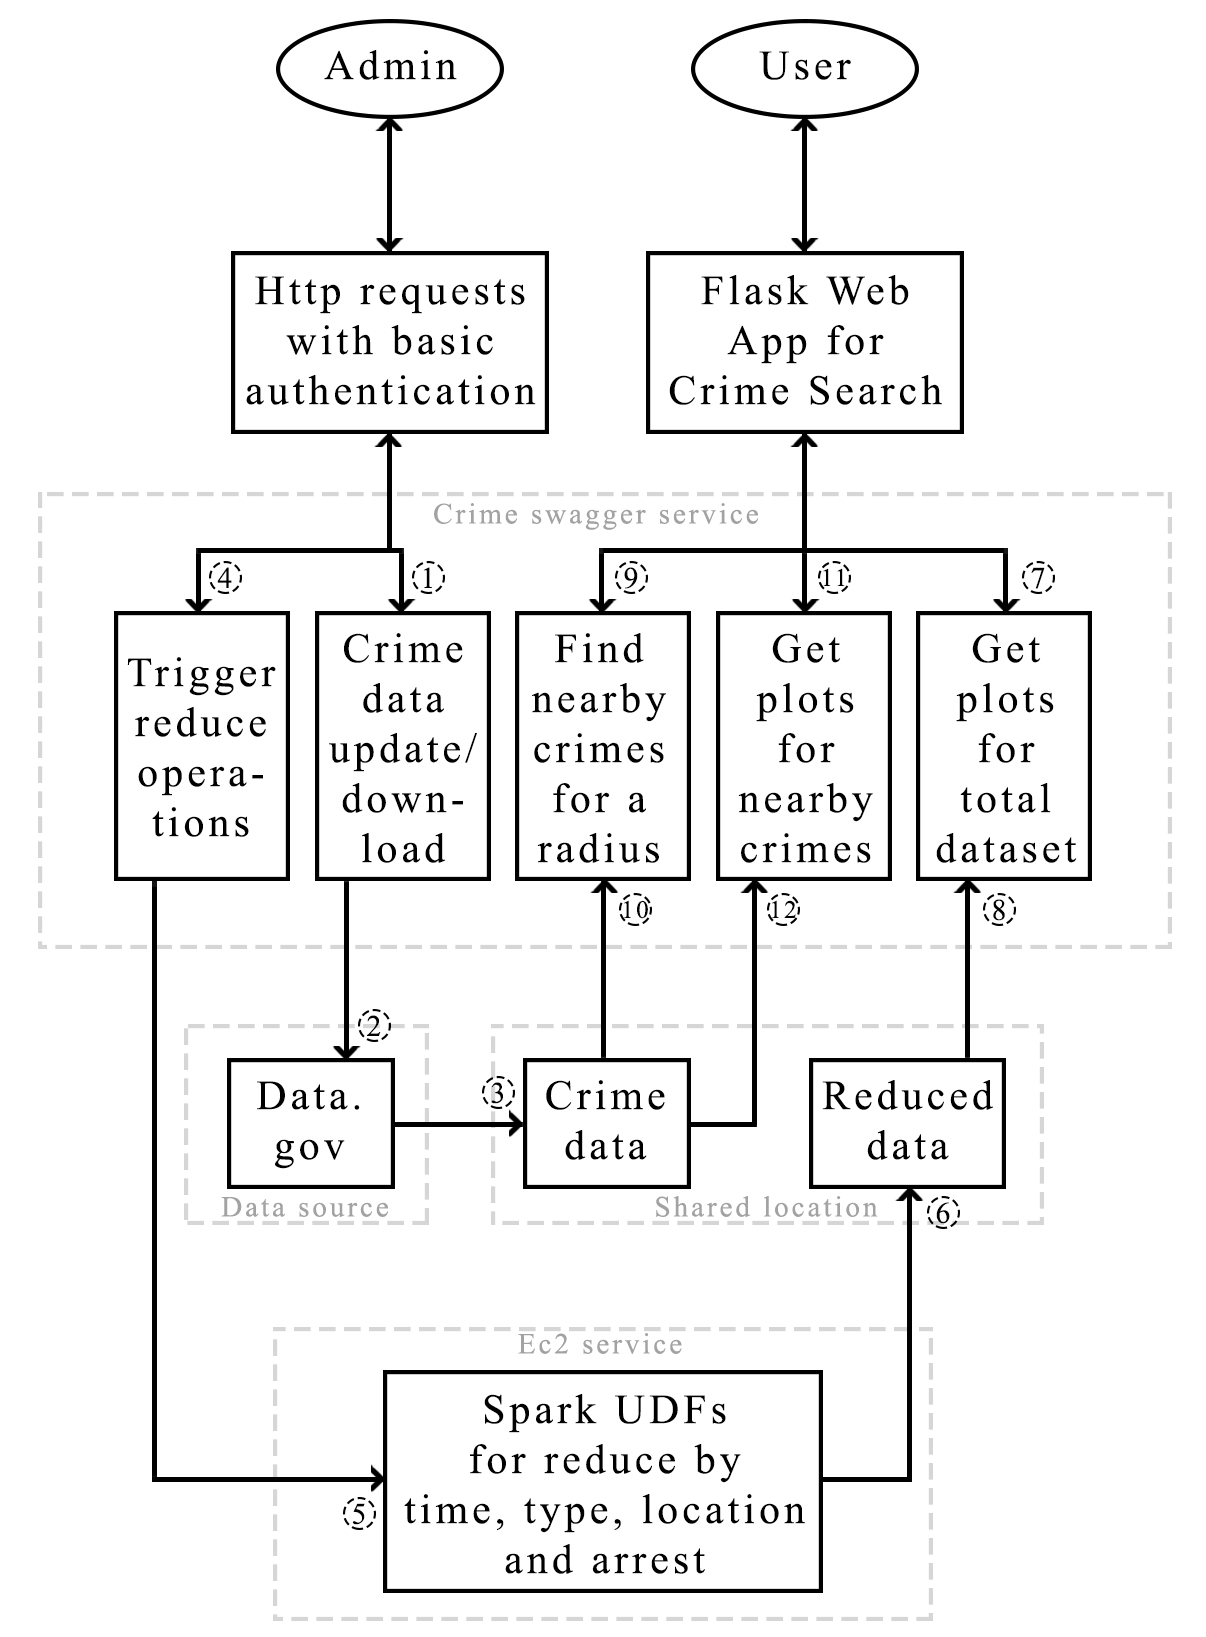
\includegraphics[width=\columnwidth]{../images/overview.jpg}
	\caption{Overview of suggested framework for crime data analysis}
	\label{fig:overview}
\end{figure}

\subsection{Data Acquisition}



Attribute Information about dataset are as follows:
\begin{itemize}
	\item ID : Unique identifier for the record.
	\item Case Number : The Chicago Police Department RD Number.
	\item Date : Date when the incident occurred.
	\item Block : The partially redacted address where the incident occurred.
	\item IUCR : The Illinois Unifrom Crime Reporting code. 
	\item Primary Type : The primary description of the IUCR code.
	\item Description : The secondary description of the IUCR code.
	\item Location Description : Description of the location where the incident occurred.
	\item Arrest : Indicates whether an arrest was made or not.
	\item Domestic : Indicates whether the incident was domestic-related as defined by the Illinois Domestic Violence Act.
	\item Beat : Indicates the beat where the incident occurred.
	\item District : Indicates the police district where the incident occurred.
	\item Ward : The ward where the incident occurred.
	\item Community Area : Indicates the community area where the incident occurred.
	\item FBI Code : Indicates the crime classification as outlined in the FBI's National Incident-Based Reporting System (NIBRS).
	\item X Coordinate : The x coordinate of the location where the incident occurred. This location is shifted from the actual location for partial redaction but falls on the same block.
	\item Y Coordinate : The y coordinate of the location where the incident occurred. This location also is shifted from the actual location for partial redaction but falls on the same block.
	\item Year : Year the incident occurred.
	\item Updated On : Date and time the record was last updated.
	\item Latitude : The latitude of the location where the incident occurred.
	\item Longitude : The longitude of the location where the incident occurred. 
	\item Location - The location where the incident occurred in maps format.
\end{itemize}

\subsection{preprocessing}

Null Value Treatment

Date time conversion

\subsection{Technology Usage}
Following programming environments and library packages were  used to implement the crime analyzing and visualization framework. 
\begin{itemize}
	\item Python 3.6 programming environment
	\item Flask 0.12
	\item connexion 1.1.15
	\item decorator 4.2.1
	\item python-dateutil 2.6.0
	\item setuptools 21.0.0
	\item numpy 1.14.0
	\item scipy 0.18.1
	\item pandas 0.20.3
	\item scikit-learn 0.18
	\item pyspark W2.1.1
	\item java 8.0 run time environment
	\item Apache Spark standalone version
	\item Swagger codegen libraries
	\item HTML 5
	\item CSS
	\item Java Script
	\item JQuery
	\item Google Maps Java script API
\end{itemize}

\subsection{Spark Map Reduce module for crime analysis using time, type and location}

\subsection{Swagger web service for location based Crime analysis}

\subsection{Flask web application for visualization}

\section{Results and Benchmarking}

\subsection{Infrastructure description}

\subsection{Performance analysis}
Training Time breakdown, 
Data cleaning time breakdown, 
system set up time, 
time taken to system launch.

\section{Discussion} 

\section{Conclusion} 

\begin{acks}
	
The authors would like to thank Dr.~Gregor~von~Laszewski for his
support and suggestions to write this extended abstract.
	
\end{acks}

\bibliographystyle{ACM-Reference-Format}
\bibliography{report} 
